%Praesentationsmodus
\documentclass[t,aspectratio=169,divpsnames]{beamer}
%Die Beameroption aspectratio legt das verwendete Seitenverhaeltnis fest
%aspectratio=169	16:9 Seitenverhaeltnis
%aspectratio=1610	16:10 Seitenverhaeltnis
%aspectratio=43		4:3 Seitenverhaeltnis
%Die Beameroption envcountsect nummeriert Umgebungen wie theorem pro section durch.
%Die Beameroption divpsnames wird an das xcolor Paket durchgereicht.

%Handout-Generierung mit Foliennotizen (statt obiger Zeile für den Präsentationsmodus verwenden)
%\documentclass[t,handout,aspectratio=169]{beamer}
%\setbeameroption{show notes}

\usepackage[utf8]{inputenc}

% Deutsch
%\usepackage[ngerman]{babel} 
%\usepackage{bibgerm}

% Englisch
\usepackage[english]{babel}

\mode<presentation>
{
\usetheme{HochschuleTrier}
\setbeamercovered{transparent}
}

%\usepackage{mathptmx}
%\usepackage[scaled=0.9]{helvet}
\usepackage{helvet}
\usepackage{courier}
%\usepackage{ae}

\usepackage{hyperref}
\usepackage{tikz}
\usepackage{amsmath}
\usepackage{amsfonts}

\logo{
\includegraphics[height=20.5mm]{UniKonstanz_Logo_Optimum.pdf}}

\usetikzlibrary{calc,positioning}

\usefonttheme[onlymath]{serif}

\usepackage{listings}
\usepackage{tikz}
\usepackage{lipsum}
\usepackage{listings}
\usepackage{xcolor}
\usepackage{siunitx}

\definecolor{codegreen}{rgb}{0,0.6,0}
\definecolor{codegray}{rgb}{0.5,0.5,0.5}
\definecolor{codepurple}{rgb}{0.58,0,0.82}
\definecolor{backcolour}{rgb}{0.95,0.95,0.92}

\long\def\/*#1*/{}

\lstset
{
	basicstyle=\ttfamily, 
	keywordstyle=\color{blue}\bfseries\ttfamily,
	identifierstyle=\ttfamily, 
	stringstyle=\ttfamily,
	commentstyle=\color{ForestGreen},
	showstringspaces=false,
	framexleftmargin=7mm, 
	breaklines=true,
	tabsize=3,
	showtabs=false,
	frame=single, 
	rulesepcolor=\color{blue},
	numbers=left,
	linewidth=146mm,
	xleftmargin=8mm,
	language={C++},
}
% Stil des Literaturverzeichnisses
\bibliographystyle{geralpha}
%\bibliographystyle{alpha}
%\bibliographystyle{abstract}

%Bitte ausfuellen:
\title{Immersive Analytics}
\subtitle{Slides for the Course}
\author{Felix Kalchschmid}
\institute{Universität Konstanz}
\date{02.11.2023}
\subject{Immersive Analytics with Applications in the Life Sciences}

%Inhaltsverzeichnisses bis auf subsubsection-Ebene:
%\setcounter{tocdepth}{3}

%Aktivieren, um am Anfang jeder Section ein Inhaltsverzeichnis zur Section anzuzeigen
%\AtBeginSection[]
%{
%\begin{frame}<beamer>
%\frametitle{Agenda}
%\tableofcontents[currentsection,hideothersubsections,sectionstyle=show/hide,subsubsectionstyle=show/show]
%\end{frame}
%}

%Aktivieren, um alles Schritt-fuer-Schritt einzublenden
%\beamerdefaultoverlayspecification{<+->}

\begin{document}

\begin{frame}
\titlepage
\end{frame}

\begin{frame}
\frametitle{Agenda}
\tableofcontents
%\tableofcontents[hideallsubsections] % Subsections ausblenden
%\tableofcontents[pausesections] %Sections Schritt-fuer-Schritt einblenden
\end{frame}

\section{Session 1}
\begin{frame}{Question 1}{Software/framework/library supporting data analytics in IE or building IA applications}
\begin{itemize}
    \item Chosen Software: CesiumJS
    \item What can it do?: 3D globes \& 2D map creation in browsers; geospatial visualization
    \item Benefits over traditional tools: 
    \begin{itemize}
        \item Plugin-free browser support, can be integrated into game engines, Uses WebGL for smooth graphics
        \item Open Platform with a lot of geospatial data available
        \item Time-dynamic visualization
        \item Open-source (commercial) \& community-driven
    \end{itemize}
    \item Expected improvement for analysis: Enhanced geospatial data visualization capability, allowing for real-time dynamic analyses. Provides an immersive experience for users, aiding in better understanding and interpretation of data.

\end{itemize}
\end{frame}
\begin{frame}{Question 2}{two opportunities that IA offers beyond visual analytics + personal example}
\begin{enumerate}
    \item open ended exploration vs. analytical applications grounded in the real world.
        \begin{itemize}
    \item overview first, zoom and filter, then details on demand.

    \item detailed information on objects in physical environment $\leftarrow$ context info on demand
\end{itemize}
    \item abstract data better visualized in 2D vs. 3D (valid in immersive environments?) 
    \begin{itemize}
    \item 2D: No occlusion, clear layout of data
    \item 3D: no inherent spatial information, occlusion, perspective, etc. 
    \item Benefits for multidimensional data? Benefits of IE?
\end{itemize}
    \item Open-Ended Exploration: Example from my life /data analysis:
            \begin{itemize}
    \item zooming into the world on google maps
    \item globe $\rightarrow$ map of country with biggest cities $\rightarrow$ local view with streets $\rightarrow$ detailed local view with restaurants $\rightarrow$ 3d view with mapped reconstructed satellite images $\rightarrow$ street view with actual photos
    
\end{itemize}
\end{enumerate}


\end{frame}

\begin{frame}{Question 3}{one interesting IA aspect from the papers}
\begin{itemize}
    \item Chosen Aspect: Multi-Modal representation and interaction.
    \item Description: Haptics and Data Physicality as well as sonification through audio can improve the experience of interacting with the data and make it feel more natural.  
    \item Interesting: Important for enabling non-visual data inputs (impairments, multi-sensory input), Many haptic-feedback devices have been developed. Audio feedback can improve immersion, builds on already learned patterns.
    \item Challenging: inferior to real touch, none of the haptic-feedback devices is perfect. 
\end{itemize}
\end{frame}

\section{Session 2}
\begin{frame}{Session 2}
    
\end{frame}
\section{Session 3}
\begin{frame}{Session 3}
    
\end{frame}
\section{Session 4}

\begin{frame}{Question 1}{Two devices or situations which already use a multi-sensory interface. How are they used? }
\scriptsize
\textbf{Terravision:} Interactive Globe with different view modes and the possibility to seamlessly zoom into the details up to 30 Meters distance. It has a special controller that is a combination of a giant trackball, a zoom knob.
    \begin{itemize}\scriptsize
    \item \textbf{How are they used?} Correspondence of the haptic trackball and globe movement allows instant understanding of the controls. Moving with the rotation and zooming with the knob feels natura.
    \item \textbf{same data presented via different senses:} there is no extra layer of information presented through the haptic controls, but the haptic trackball provides a more intuitive and immersive way of control.  
\end{itemize}

\begin{figure}
    \vspace{-0.1cm}
	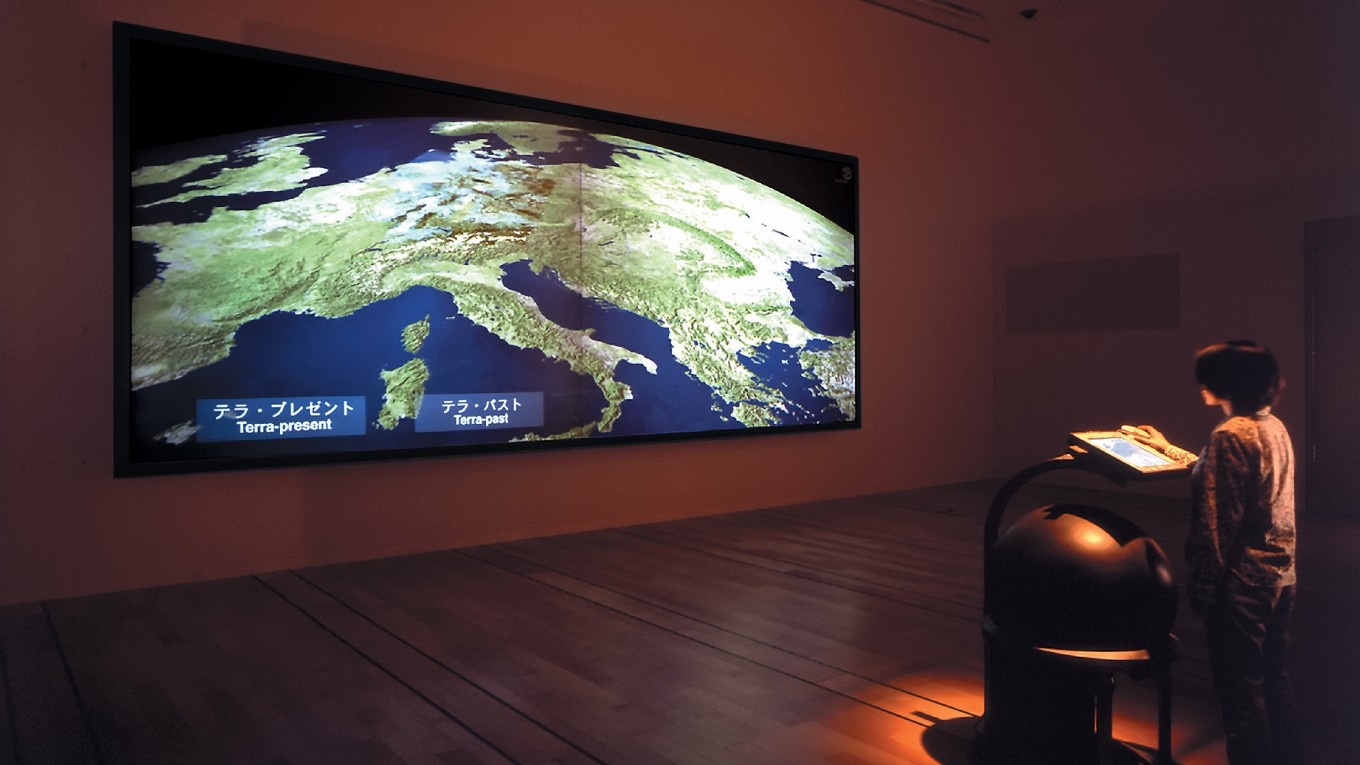
\includegraphics[width=6.5cm]{images/1996_Terravision_02-1360x765.jpg}
  \vspace{-0.3cm}

	\caption{\scriptsize Terravision: ART+COM, 1996. Globe on large screen synchronized with movement of haptic trackball controller.}
\end{figure}
\end{frame}

\begin{frame}{Question 1}{Terravision}
    \begin{figure}
    \vspace{-0.1cm}
   	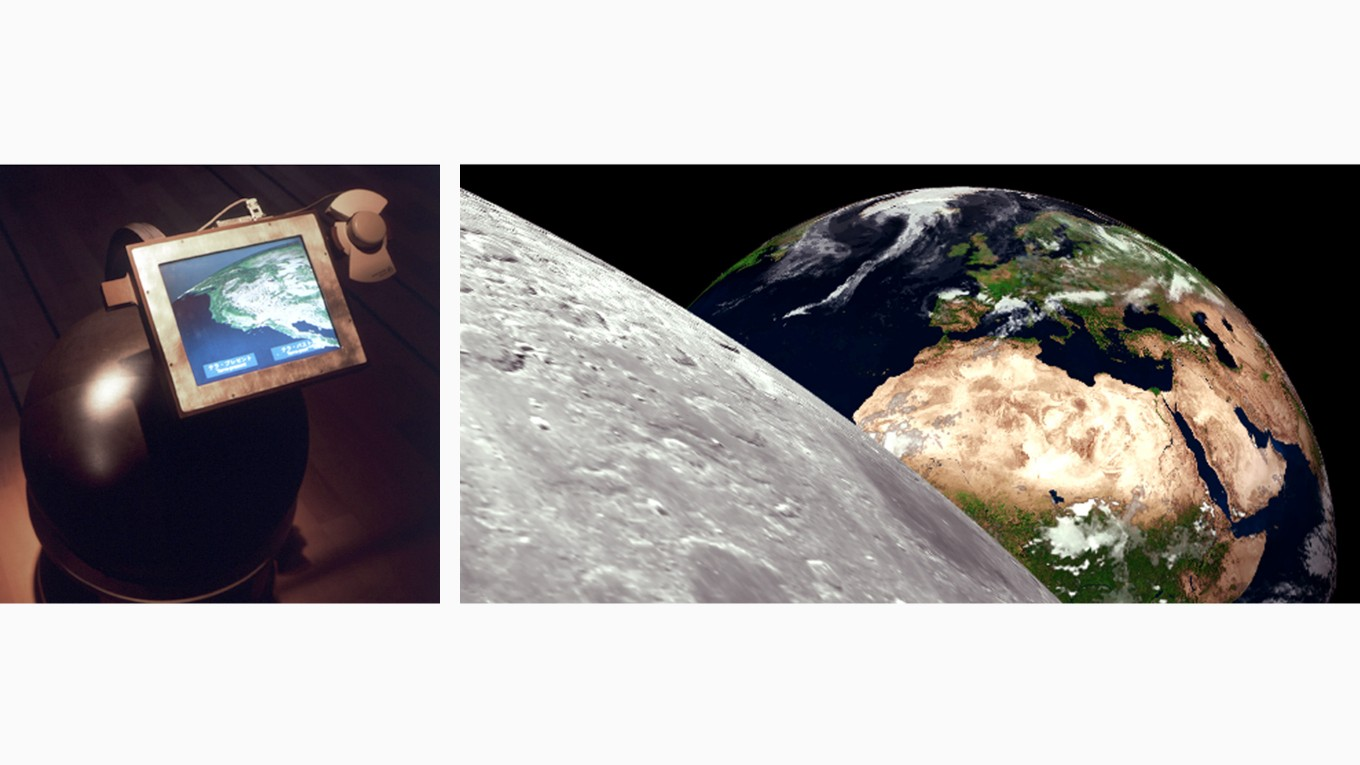
\includegraphics[width=10.5cm]{images/1996_Terravision_06-1360x765.jpg}
        \vspace{-0.9cm}

	\caption{\scriptsize Terravision: ART+COM, 1996. Trackball Controller + Cursor Knob for Zooming + Small Display}
\end{figure}
\end{frame}
\begin{frame}{Question 1}{Terravision}
    \begin{figure}
    \vspace{-0.1cm}
    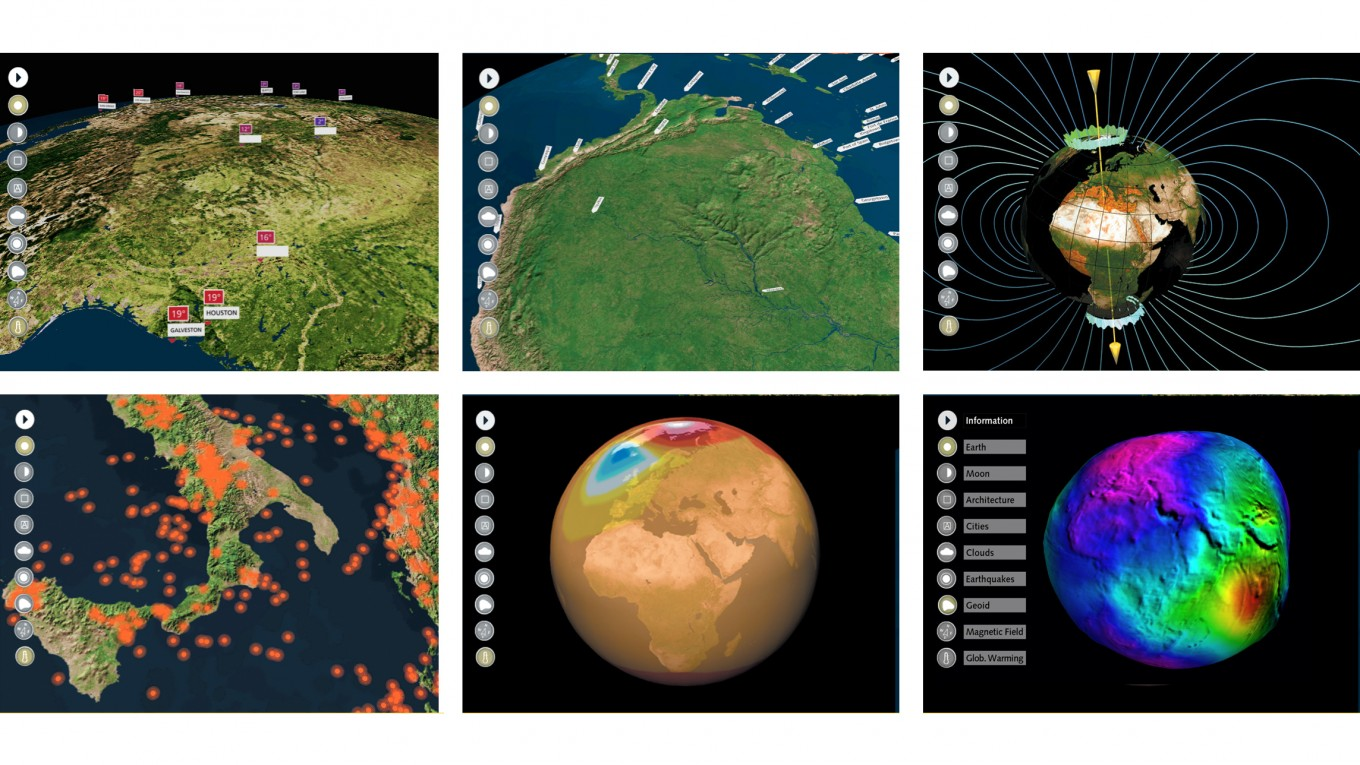
\includegraphics[width=10.5cm]{images/1996_Terravision_05-1360x765.jpg}
        \vspace{-0.7cm}
	\caption{\scriptsize Terravision: ART+COM, 1996. Different Overlay Options}
\end{figure}
\end{frame}

\begin{frame}{Question 1}{Two devices or situations which already use a multi-sensory interface. How are they used? }
\scriptsize
\textbf{Behavior tuning in public places:} Shopping in clothing and crociery stores or going to big franchise restarants is always a designed multi-sensory situation that is designed to cause or enhance certatin wanted behaviors.
    \begin{itemize}\scriptsize
    \item \textbf{Audio} - Music (how loud?, what type?) makes you spend more time get relaxed. \\%\footnote{ZARA fashion stores are known for their music} 
    Playing commercials informs people about sales and current events, no matter if they want to know.
    \item \textbf{Smell} - Always using the same scent connects feelings to memories. (causing subconcious recognition)
    \item \textbf{Haptics} - Having always the same layout in every store (ALDI) or the same food menu. Allows people to plan beforehand no matter where you are. Also the layout of stores guides the shopping behavior.
    \item \textbf{Timing of Information} - combination of persistant information displays (train station displays + paper timetable), timed audio information (loudspeaker messages in the train and on the platform), individual detailed information (DB Navigator App) allows making quick descisions based on the available information even in stressful situations. 
\end{itemize}
\end{frame}



\begin{frame}{Question 2}{Example for each column in the design framework for multisensory immersive analytics}
\scriptsize
\begin{enumerate}
    \item \textbf{Data:}
    \begin{itemize}
        \item test
    \end{itemize}
    \item \textbf{Mapping:}
    \begin{itemize}
        \item test
    \end{itemize}
    \item \textbf{Devices:}
    \begin{itemize}
        \item test
    \end{itemize}
    \item \textbf{Human:}
    \begin{itemize}
        \item test
    \end{itemize}
\end{enumerate}


\end{frame}

\begin{frame}{Question 3}{Three acoustic attributes. Explain one of them. Can they be used in a similar way, e.g. compared to visual variables?}
\scriptsize
\begin{enumerate}
    \item \textbf{Pitch:}
    \item \textbf{Loudness:}
    \item \textbf{Timbre:}
    \item \textbf{Location:}
    \item \textbf{Musical components:}
\end{enumerate}
\textbf{Usage compared to visual variables:}
\scriptsize
\begin{itemize}
    \item test
\end{itemize}
\end{frame}


\section{Project Description}
\begin{frame}{Project Description}{Augmented Reality for Geospatial Land-Use Data Visualization}
The objective is an Augmented Reality (AR) project designed to optimise the interaction with and understanding of geospatial land use data. By integrating 3D representations of land use, in the form of procedurally generated plant models, with Cesium map data, this project aims to provide a comprehensive, intuitive and interactive visual exploration of geographic landscapes and their changes over time. This tool could be particularly valuable for applications in urban planning, environmental monitoring, and policy-making regarding infrastructure development such as highways or forestry management.
\end{frame}
\begin{frame}{Project Description}{Use-Case}
The application serves multiple purposes:
\begin{itemize}
    \item \textbf{Time-based Comparison:} Observing changes in specific areas over time, enabling trend analysis and future projections.
    \item \textbf{Behavioral Analysis in Specific Areas:} Understanding patterns in certain geographic patches and extrapolating these insights to similar regions.
    \item \textbf{Supporting Political Decision-Making:} Assisting in choices related to infrastructure development, forestry conservation, and other geospatially reliant political decisions.
\end{itemize}
\end{frame}
\begin{frame}{Project Description}{Intended Features}

\scriptsize
\begin{enumerate}
    \item \textbf{3D Visualization:} Utilizing Cesium map data to create a 3D world where land use is represented through detailed 3D models of vegetation and terrain.
    \item \textbf{Interactive Environment:} Users can interact with the virtual landscape to reveal specific data about land use.
    \item \textbf{Augmented Reality Integration:} Displaying a section of the land on a real table in real space, enhancing the sense of immersion and understanding.
    \item \textbf{Dynamic Data Presentation:} Abstract data about land use is showcased on a virtual screen, tailored to the user's focus within the environment.
    \item \textbf{Interactive 2D Map:} A complementary feature where users select locations for detailed 3D exploration.
    \item \textbf{Neighboring Tiles Interaction:} Smooth transition between adjacent areas in the 3D representation, enhancing the spatial understanding of the region.
    \item \textbf{Direct Visualization of Influencing Factors:} Displaying factors like overshadowing directly through the visualization's inherent properties.
    \item \textbf{Non-interpretative Comparison:} Offering a comprehensive view of the area without the need for data interpretation.
    \item \textbf{Plant Simulation:} Interactive simulation of plant growth and interaction within the environment.
    \item \textbf{Intuitive Data Representation:} Visual representations that inherently express their characteristics, making data interpretation more intuitive.
\end{enumerate}
\end{frame}
\begin{frame}{Project Description}{Minimum Outcome}
Best to be implemented with a augmented reality HMD using Unity and Cesium
\begin{itemize}
    \item A 3D parcel of land showcasing land use data through color-coded highlights and 3D models of local flora.
    \item Two modes of display: Flat (2D) and side view for direct data representation from the database.
    \item Placement of this 3D parcel on a real-world table for enhanced interaction and understanding.
    \item Multi-user functionality for collaborative analysis and decision-making (if time permits).
\end{itemize}

%This project, with its focus on interactive, intuitive, and comprehensive data visualization, is poised to make significant contributions to the fields of urban planning, environmental monitoring, and political decision-making, fostering a deeper understanding of our world's geographical intricacies.
\end{frame}

\begin{frame}{Project Description}{What other senses could it support? Which data to present to these? How would it be presented?}
\scriptsize
\begin{enumerate}
    \item \textbf{Other sense to support:}
    \item \textbf{Data to present to it:}
    \item \textbf{Way to present data:}
\end{enumerate}

\end{frame}



\begin{frame}{Conclustion}{Summary}

\end{frame}
\section*{End}
%\begin{frame}
%	\begin{center}
%		\huge{Thank you for your attention.}
%	\end{center}
%	\begin{center}
%		\Huge{Questions?}
%	\end{center}
%\end{frame}

\begin{frame}[allowframebreaks]{\bibname}
\bibliography{literatur}     %BibTeX-Datei literatur.bib
\end{frame}


\end{document}
